\chapter{Forskningsprojekt}\label{forskning}

\begin{center}
	~ \\[0.5cm]
	
\noindent\makebox[\linewidth]{\rule{\textwidth}{0.4pt}}\\
[0.5cm]{\LARGE Forskningsprojektet har til formål at undersøge betydningen for det nødvendige fraktureringstryk i 3D-printede aortarødder med varierende kalcificeringsgrad}
\noindent\makebox[\linewidth]{\rule{\textwidth}{0.4pt}}

	~ \\[0.5cm]	


\begin{figure}[H]
	\centering
	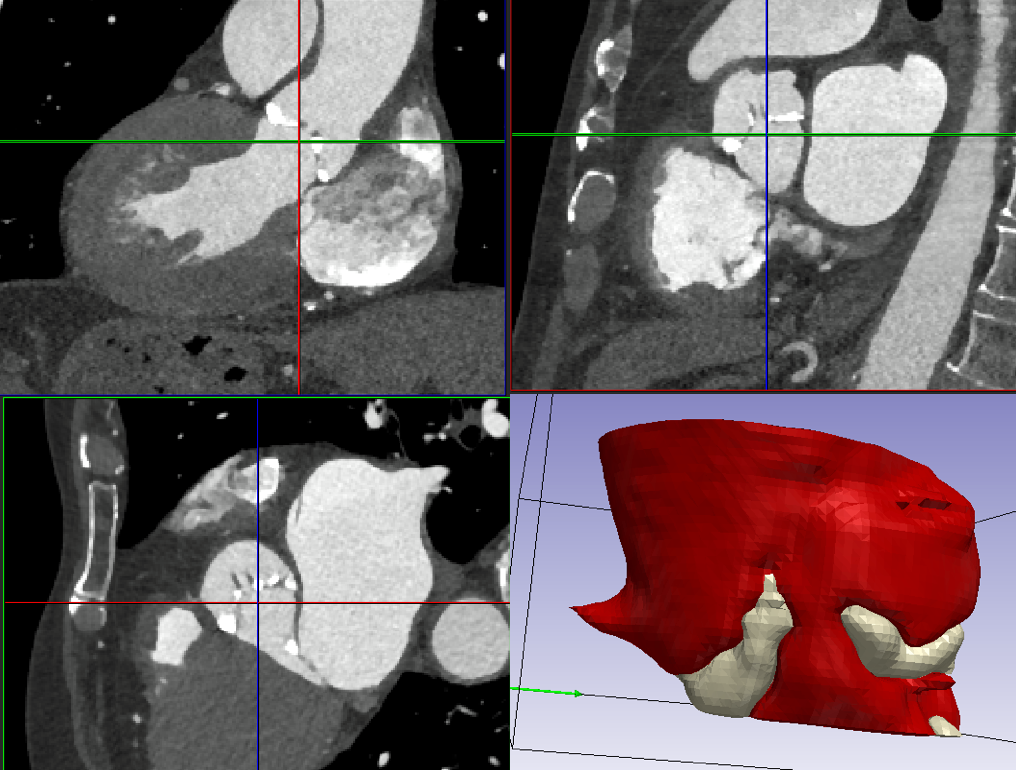
\includegraphics[width=1\textwidth]{Figure/forside}
\end{figure} 


\end{center}

\clearpage

\section{Introduktion} 

I dag bliver biologiske hjerteklapper valgt til fordel for de mekaniske hjerteklapper ved hjerteklapsudskiftninger \cite{baggrund10}. Ulempen ved dette valg er, at levetiden for de biologiske hjerteklapper er reduceret og patienterne skal ofte have en reoperation. Her har ViV teknikken vist sig som et lovende alternativ til åben hjertekirurgi \cite{baggrund10}. ViV teknikken er særligt at foretrække hos højrisiko patienter, hvor åben hjertekirurgi ikke er hensigtsmæssig. ViV teknikken bygger på TAVI proceduren, hvor den biologiske hjerteklap bliver indsat gennem et kateter og implanteret i den degenererede hjerteklap.  

ViV teknikken har på nuværende tidspunkt sine begrænsninger ved små biologiske hjerteklapper (19 mm og 21 mm), hvormed proceduren ikke er hensigtsmæssigt at udføre. Små biologiske hjerteklapper har et mindre åbningsareal end, hvad der er ønskværdigt for, at proceduren kan udføres. At udføre ViV ved en lille biologisk hjerteklap vil derfor reducere det effektive åbningsareal ydeligere og sandsynligvis have en negativ effekt på den postoperative trykgradient, hvormed det kliniske resultat ikke er optimalt \cite{baggrund22}\cite{baggrund10}. 

Der er for nyligt forsket i en ny metode, BF-ViV, som potentielt kan løse problematikken med for små biologiske hjerteklapper. Metoden indebærer frakturering af den degenererede biologiske hjerteklap, hvormed det effektive åbningsareal øges. Herefter kan en ny biologisk hjerteklap indføres ved den tidligere nævnte ViV teknik.  

Tidligere i forskningen er det blevet undersøgt, hvorvidt forkalkning af aortaroden har indflydelse på det nødvendige fraktureringstryk. Studiet viste, at der er en signifikant forskel på 3D-printede aortamodeller uden forkalkning og 3D-printede aortamodeller med total annulær forkalkning af annulus \cite{rapport}. 

Forkalkning af aorta er en degenerativ sygdom og forkalkningsmængden vil være specifik for den pågældende patient. På baggrund af patientspecifikke CT scanninger er det påvist, at graden af kalk varierer hos patienter med aortastenose, se Forstudie 2.1 i dokumentationen afsnit 9.6. Det vil derfor være relevant at undersøge, hvorledes den varierende kalkmængde har indflydelse på det nødvendige fraktureringstryk. Der er til dette studie produceret 3D-printede aortamodeller, hvor kalken er systematisk fordelt med henholdsvis 0\%, 25\%, 50\%, 75\%, 95\% og 100\% kalk, se Forstudie 2.2 i dokumentationen afsnit 9.7. Formålet med dette studie er derfor at undersøge det nødvendige fraktureringstryk ved de forskellige 3D aortamodeller.        

\section{Metode og materiale} 
I det følgende afsnit vil metode- og materialevalg til udførsel af studiet beskrives. Endvidere vil de statistiske metodeovervejelser præsenteres. 
 
\subsection*{Metode for udførsel} 
Forsøgene blev udført i CAVE lab på Aarhus School of Engineering, Aarhus Universitet. Til at udføre og måle de aktuelle fraktureringer anvendes det udviklede detekteringssystem. På Figur \ref{opstilling} ses en illustration af forsøgsopstillingen. 

\begin{figure}[H]
	\centering
	\includegraphics[width=1\textwidth]{Figure/Delstudie2opstilling}
	\caption{Illustration af forsøgsopstillingen }
	\label{opstilling}
\end{figure} 
 
Inflator med påmonteret manometer (EAGLE\texttrademark \ Inflation device, Bard Medical, USA) samt True\texttrademark \ Dilatation ballon, 22 mm (Bard Peripheral Vascular, Inc., Tempe, AZ, USA) monteres i specialfremstillet holder og tilkobles begge til trevejshane 1. Omkring True\texttrademark \ Dilatation ballon er en POM-stent (indre diameter: 17.3mm, ydre diameter: 19.3 mm, tykkelse: 1mm, boret 0.7 mm hul) samt 3D aortamodel med ønsket kalkmængde (0\%, 25\%, 50\%, 75\%, 95\% eller 100\%) placeret. Hullet i POM-stenten er placeret ved kalken, da det er her fraktureringen sker og det er påvirkningen af kalken, der ønskes undersøgt. 

Inflatoren fyldes med vand via trevejshane 2. Det er vigtigt at sikre, at forsøgsopstillingen er fri for luftbobler. Hvis dette ikke er tilfældet lukkes samme hane op og luften presses ud, indtil vand løber ud af hanen. Ved manuelt at dreje langsomt på inflatoren inflateres ballonen med vand og trykket øges langsomt som funktion heraf. Tryktransduceren (Pressure Transmitter, AKS 32, Danfoss - Nordborg, DK) er forbundet til trevejshane 2 og er forsynet med 18 V indgangsspænding fra to 9 V batterier. Tryktransduceren måler det aktuelle tryk i ballonen og er tilkoblet DAQ'en (NI USB-6009 8inputs, 14-bit, multifunction I/O, Austin, TX, USA), som konverterer trykket til et digitalt signal.

Det digitale signal indlæses og behandles i det udviklede detekteringssystems software. Der er til udførelse af dette studie tilføjet en gem-funktion til detekteringssystemet, hvor signalet udskrives og gemmes lokalt som en Excel fil på computeren. Denne funktion skal verificere, at det udskrevende faktureringstryk på detekterings GUI'en stemmer overens med det aflæste i Excel filen.  
 
Udviklingen af 3D aortamodeller er dokumenteret i Forstudie 2.1 og 2.2 afsnit 9.6 og 9.7. 
Gennem Forstudie 2.1 blev patientspecifikke CT scanninger segmenteret, hvorfra 3D-printede aortamodeller med forskellige kalcificeringsgrader blev produceret. De forskellige kalcificereringsgrader gav anledning til, at opdele de producerede 3D-printede aortamodeller i tre kategorier: let-, moderat- og svær forkalkning. Se dokumentation afsnit 9.6.2 for beskrivelsen af disse kategorier. Disse 3D-printede aortamodeller levede ikke op til forventningerne og kunne ikke anvendes, se dokumentation afsnit 9.6.5.   

Gennem Forstudie 2.2 blev cirkulære 3D-printede aortamodeller med forskellige kalcificeringsgrader produceret. Den cirkulære geometri blev valgt for at sikre den bedst mulige fitting og dermed undgå luft mellem POM-stenten og aortamodellen. 

Modellerne er fremstillet i materialet TangoBlackPlus (Shore 27A) \cite{Datablad_Damvig}, som ofte bruges til fremstilling af hjertemodeller \cite{tangoplus}. Det er derfor valgt at bruge dette materiale til fremstilling af aortamodellerne. Materialet VeroWhitePlus (Shore 83D) \cite{Datablad_Damvig} er tidligere brugt i kombination med TangoPlus til at fremstille aorta stenoserede modeller \cite{rapport}. Det blev derfor valgt, at bruge dette materiale til simulering af kalk. De printede 3D aortamodellerne ses på Figur \ref{alle_systematisk}.   
 
 \begin{figure}[H]
	\centering
	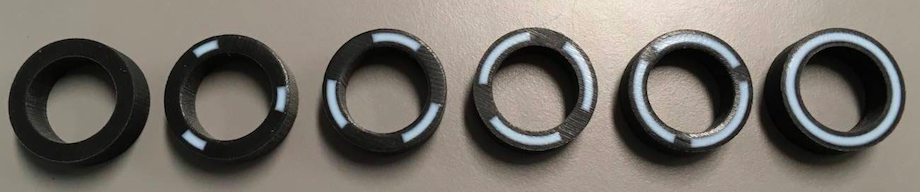
\includegraphics[width=0.8\textwidth]{Figure/alle_systematisk}
	\caption{3D aortamodeller med varierende kalkmængder}
	\label{alle_systematisk}
\end{figure} 
 
\subsection*{Statistisk metode}
Statistisk ønskes det undersøgt, hvorledes de forskellige kalcificeringsgrader muligvis påvirker det nødvendige fraktureringstryk. Hvilken statistisk metode der bør anvendes, skal afgøres som flowdiagrammet på Figur \ref{flow} antyder. 

\begin{figure}[H]
	\centering
	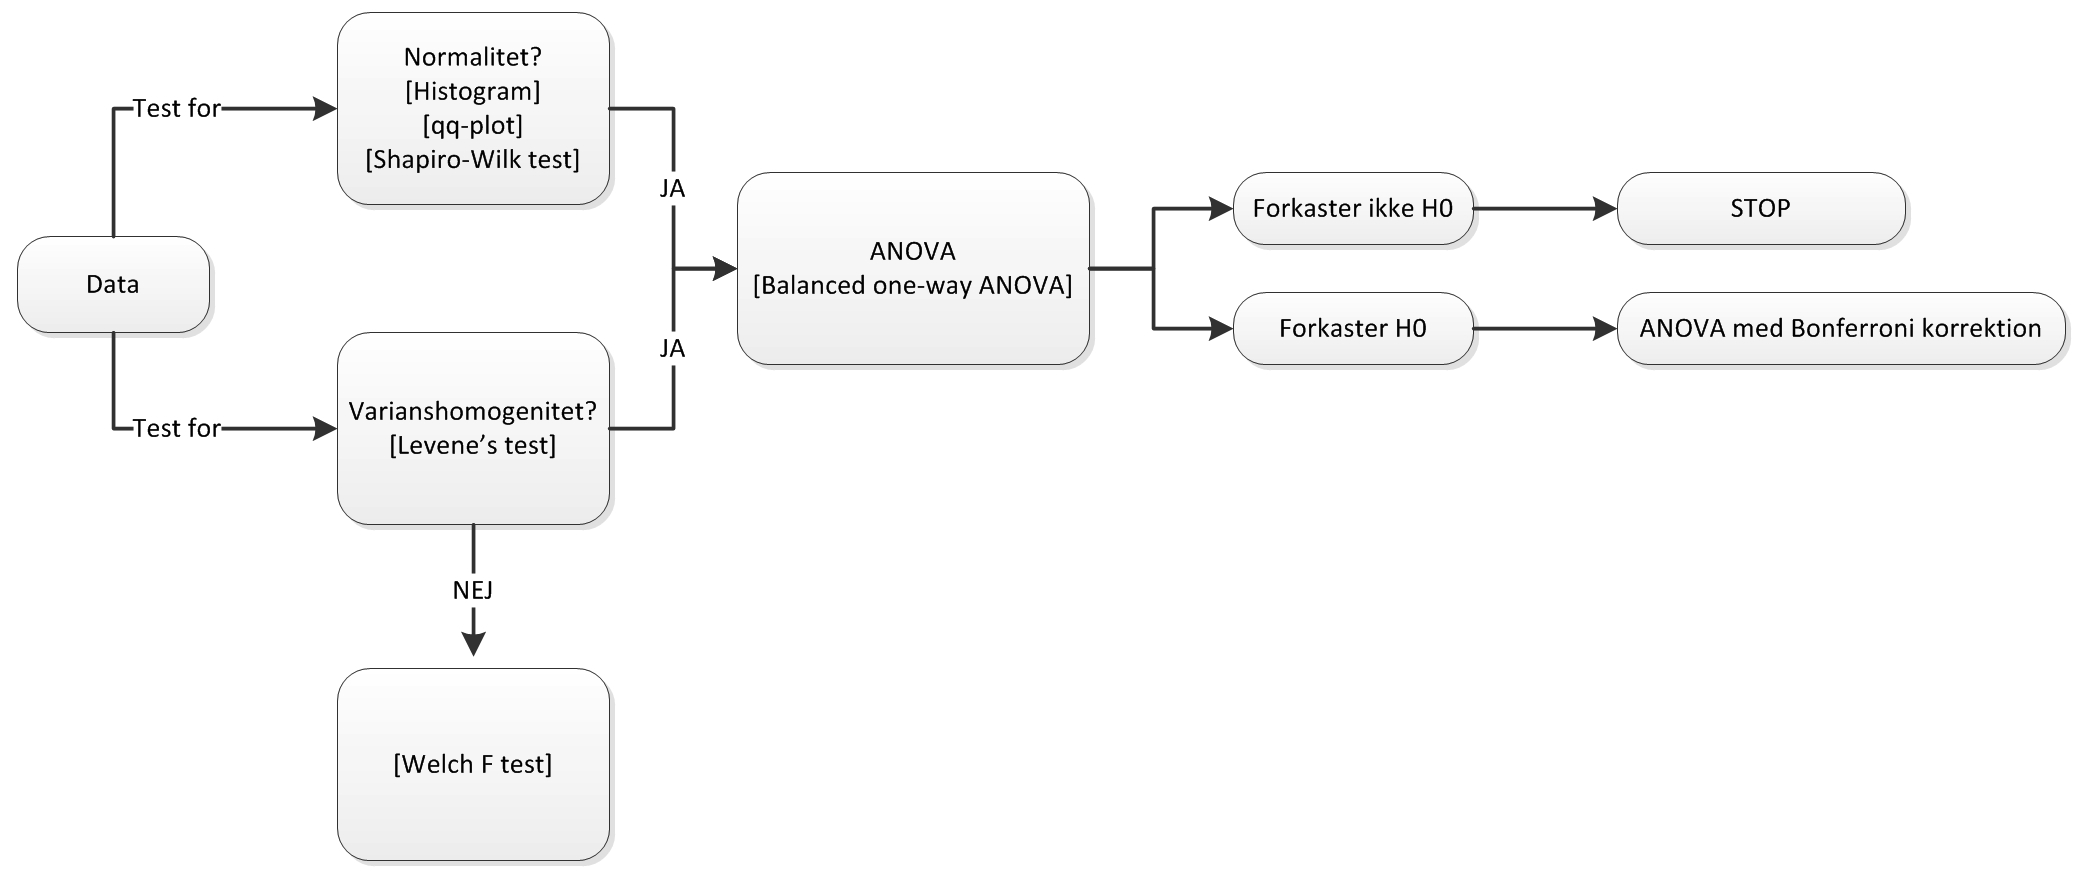
\includegraphics[width=1\textwidth]{Figure/statistiskmetode}
	\caption{Flowdiagram, der illustrerer fremgangsmåden for valg af statistisk metode. Normalitet er også en forudsætning for anvendelsen af Welch F test}
	\label{flow}
\end{figure}  

Grundlæggende ønskes den statistiske metode analysis of variance (ANOVA) anvendt, da den tester, hvorledes middelværdierne i mere end to grupper er ens. Før ANOVA kan anvendes skal data testes for normalitet samt varianshomogenitet, da disse er antaget, der skal være tilstede før ANOVA kan benyttes. Hvis disse antagelser accepteres udføres balanced one-way ANOVA. Forkastes nul-hypotesen ikke kan det ikke afvises, at middelværdierne mellem grupperne er ens. Omvendt hvis nul-hypotesen forkastes, vil mindst én af gruppernes middelværdier være statistisk signifikant forskellige fra de andre. For at bestemme hvilken/hvilke gruppe(r), der er forskellige fra hinanden benyttes den statistiske metode ANOVA med Bonferroni korrektion.

Hvis antagelsen om ens varians ikke kan accepteres, kan metoden Welch F test benyttes istedet for \cite{welchftest}. 
  

\section{Resultater}
Der blev udført fem fraktureringer i 3D aortamodellerne 0\% til 95\%, hvor der kun blev udført én i 3D aortamodellen med 100\% kalk. Resultaterne for det nødvendige fraktureringstryk ses i Tabel \ref{radata} samt i Bilag 9.


\begin{table}[H]
	\centering 
		\resizebox{\textwidth}{!}{\begin{tabular} {@{}lccc@{}}
		\toprule
& \textbf{Obs.} & \textbf{Middel frakturtryk} & \textbf{Std. afv.}\\ \midrule
\textbf{3D-printet aortamodel med 0\% kalk} & 5 & 8,82 & 0,81\\
\textbf{3D-printet aortamodel med 25\% kalk} & 5 & 8,32 & 0,60\\
\textbf{3D-printet aortamodel med 50\% kalk} & 5 & 8,54 & 0,32\\
\textbf{3D-printet aortamodel med 75\% kalk} & 5 & 8,22 & 0,39\\
\textbf{3D-printet aortamodel med 95\% kalk} & 5 & 8,88 & 0,45\\
\textbf{3D-printet aortamodel med 100\% kalk} & 1 & 13,3* & -\\
	\bottomrule
	\multicolumn{4}{@{}l}{\footnotesize * Udført blot én frakturering ved 100\% kalcificering, da ballonen sprang ved 13,3 atm. POM-stenten frakturerede ikke.  }\\
	\multicolumn{4}{@{}l}{\footnotesize Alle tryk er opgivet i atm.}\\
	\end{tabular}}
	\caption{Resultat af det nødvendige middel fraktureringstryk ved de forskellige 3D modeller med varierende kalcificering}
	\label{radata}
\end{table}

Ud fra resultaterne tyder det på, at tilstedeværelsen af kalk mellem 0\% - 95\% ikke har den store betydning for det nødvendige fraktureringstryk. For at kunne underbygge denne teori foretages statistiske beregninger af data. For at afgøre hvilken statistisk model der kan anvendes, følges flowdiagrammet, se Figur \ref{flow}. 

For at teste om data er normalfordelte, er der blevet lavet histogrammer, qq-plots og Shapiro-Wilk test for hver gruppe, se resultaterne for de forskellige tests i Bilag 10. Grundet lille sample size kan det ikke udfra histogrammerne og qq-plots konkluderes om data er normalfordelte. Resultatet af Shapiro-Wilk testen er en p-værdi, som giver en statistisk sandsynlighed på 95\% om, hvorvidt data er normalfordelte. Resultaterne viste, at det ikke kan afvises, at data er normalfordelte, da p-værdierne er >0,05. 

For at teste om data har varianshomogenitet udføres Levene's test. Hvis p-værdien er >0,05 kan det ikke afvises, at data har ens varians. I dette tilfælde er p-værdien lig med 0,0474 og det kan dermed ikke konkluderes, at data har varianshomogenitet. Den statistiske metode ANOVA kan dermed ikke anvendes. 

Istedet anvendes en Welch F test, som ud fra artiklen \cite{welchftest} har vist sig at være den bedste statistiske metode til at teste for ens middelværdi mellem flere grupper, hvor variansen ikke er ens og sample size er lille. Se resultatet af Welch F test på Figur \ref{welchr} samt i Bilag 10.

\begin{figure}[H]
	\centering
	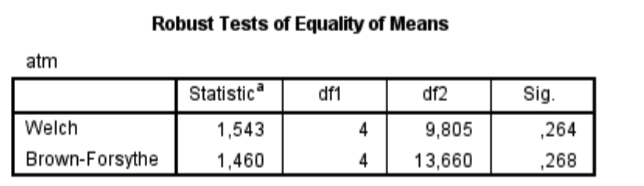
\includegraphics[width=1\textwidth]{Figure/welch}
	\caption{Resultat af Welch F test udført i SPSS (da STATA ikke havde denne funktion)}
	\label{welchr}
\end{figure}

Welch F test giver en p-værdi på 0,264, hvilket er >0,05, hvormed nul-hypotesen om, at middelværdierne mellem grupperne er lig med hinanden, ikke kan afvises. 
  

\section{Diskussion}

\subsection*{Sample size}
Sample size for dette studie er på 25 og tænkes at være for lille. Årsagen til, at Levene's test giver en p-værdi <0,05, kan være grundet den lille sample size og årsag til, at den statistiske metode ANOVA ikke kunne anvendes. En sample size beregning med en power på 0,80 ved en oneway ANOVA er blevet beregnet. Se udregningen i Bilag 10. Resultatet er en sample size på 90, altså 18 fraktureringer i hver gruppe. Dermed kan det diskuteres, hvorvidt det statistisk kan vurderes, om middelværdierne mellem grupperne er ens ved en sample size på blot 25. 

Spørgmålet om, hvorvidt forskellige kalcificeringergrader påvirker det nødvendige fraktureringstryk, bør derfor ydereligere undersøges i videre eksperimentelle forsøg.  

\subsection*{POM-stent}
Tidligere i forskningen er der blevet udviklede en POM-stent, se afsnit \ref{hojtrykssystem}, der tidligere i forskningen \cite{rapport} er verificeret til at have samme fraktureringstryk som en biologisk hjerteklap Mitroflow 21 mm. Tidligere forskning præsenterer et nødvendigt fraktureringstryk på 10 atm ved frakturering af en 3D-printet aortamodel med 0\% kalcificering aflæst på et analogt manometer. Dette nødvendige fraktureringstryk opnåes ikke i dette studie, hvor fraktureringstrykket måles via detekteringssystemet, altså via en tryktransducer. Her måles middel fraktureringstrykket, ved frakturering med en True\texttrademark \ Dilatation ballon 22mm, til 8,82 atm. 

Dermed bør sammenligningen mellem Mitroflow 21 mm og den udviklede POM-stent testes igen for at verificere det udviklede stent design, men hvor det udviklede detekteringssystem anvendes som målemetode. Hvis denne sammenligning ikke kan verificeres bør stent designet revurderes.    

\subsection*{De 3D-printede aortamodeller} 
Det vil aldrig være muligt helt nøjagtigt at efterligne aortarodens og forkalkningens komplekse fysiologiske egenskaber. Til 3D aortamodellerne har formålet været, at simulere det naturlige miljøs indflydelse på fraktureringstrykket så godt som muligt. I Forstudie 2.2, se dokumentation afsnit 9.7 og Bilag 11, er 3D aortamodellen med 0\% kalcificering printet i materialet TangoBlackPlus sammenlignet med rask griseaorta ift. det nødvendige fraktureringstryk. Disse er ens, hvilket statistiske tests underbygger, og materialet TangoBlackPlus har dermed samme indflydelse på fraktureringstrykket. På baggrund af dette vurderes det, at den 0\% kalcificerede 3D-printede aortamodel simulerer en rask griseaorta tilfredsstillende og dermed også en human aortarod. Hvorvidt VeroWhitePlus som er materialet, der skulle simulere den naturlige kalks indflydelse på fraktureringstrykket er korrekt, er mere uvist. Særligt i disse 3D aortamodeller, hvor kalken er placeret systematisk og dermed ikke ligner den virkelige morfologi. 

I tidligere forskning har det vist sig, at tilstedeværelsen af kalk har indflydelse på det nødvendige fraktureringstryk. Her blev fraktureringen foretaget i en total annulær kalcificeret patientspecifik 3D-printet aortamodel, hvor det nødvendige frakturering var 12 atm. I dette studie var det ikke muligt at bekræfte dette. En årsag hertil kan være forskellen i de anvendte 3D-printede aortamodeller. Aortamodellerne, som blev benyttet i dette studie, er cirkulære og designet, således, at der ikke forekommer luft mellem POM-stenten og aortamodellen, hvilket var tilstede ved den tidligere forskning.   

Hvorvidt de cirkulære 3D-printede aortamodeller med varierende kalk simulerer den humane kalcificerede aortarod bedre end de patientspecifikke, er fortsat usikker. Udseendemæssigt ligninger de cirkulære 3D-printede aortamodeller ikke den virkelige aortarod, men fejlkilden med luft mellem POM-stenten og aortamodellen er ikke tilstede. Hvorledes de systematisk placerede kalkaflejringer stemmer overens med, samt simulerer virkeligheden, er lidt usikke. Men udfra de opstillede kategorier i Forstudie 2.1, se dokumentation afsnit 9.6, stemmer størrelsen af de systematiske kalkaflejringer ved 25\%, 50\% og 75\% overens med kategorierne let, moderat og svær, som er kategoriseret på baggrund af patientspecifikke CT scanninger.   

I resultatafsnittet fremgår det, at mængden af kalk ved 0\%, 25\%, 50\%, 75\% og 95\% ikke har nogen betydning for POM-stentens fraktureringstryk, mens det ikke var muligt ved aortamodellen med 100\% kalk at frakturere POM-stenten. Her sprang ballonen ved 13.3 atm. Udfra dette studie tyder det på, at tilstedeværelsen af TangoBlackPlus (rask aortavæg), medfører den egenskab, at disse nemt kan strække og udvide sig i en sådan grad, at POM-stenten kan frakturere, ligegyldig kalicificeringsgraden, mens det ved 100\% kalcificering ikke er muligt at frakturere POM-stenten. Udfra Forstudie 2.1, se dokumentation afsnit 9.6, hvor forskellige patientspecifikke CT-scanninger blev studeret og segmenteret, var aortamodellen med 100\% kalicificering ikke repræsenteret. Den totale annulære forkalkning er umiddelbart ikke et scenarie, der kunne forekomme klinisk. Det blev i stedet observeret, at kalcificeringsgraderne 25\%, 50\% og 75\% ved de cirkulære 3D-printede aortamodeller bedre efterligner de patientspecifikke forkalket aortarødder.

Studiet indikere, at så længe der er rask aortavæv tilstede i patients annulus, kan der forekomme en frakturering ved samme tryk. Det vil sige, at operatøren ikke skal bekymre sig om kalcificeringsgraden, når der skal gives en forhåndsvurdering af det nødvendige fraktureringstryk. 

\section{Konklusion}  
Der er gennem segmentering af patientspecifikke CT scanninger observeret forskellige kategorier ift. kalcificingsgraden af aortaroden. For at undgå tidligere dokumenteret fejlkilde, hvor der er luft mellem POM-stenten og aortamodellen, er der blevet printet cirkulære 3D aortamodeller, hvor POM-stentens ydre diameter (19,3 mm) er 3D aortamodellens indre diameter, hvormed POM-stenten fitter aortamodellen 100\%.  

Gennem udførelsen af dette studie kan det på baggrund af de faktiske observationer samt Welch F testen konkluderes, at de forskellige kalcificeringsgrader 0\% 25\%, 50\%, 75\% og 95\% ikke har nogen indflydelse på det nødvendige fraktureringstryk. Da kalk ingen betydning har, er kalcificeringsgraden ikke en paramenter, operatøren behøver at forholde sig til ved udførelsen af proceduren, BF-ViV. Denne konklusion er dog med forbehold for lav statistisk power grundet en lille sample size.  

Det udviklede detekteringssystem blev anvendt og levede op til forventningerne. Det var muligt ved alle fraktureringer at få udskrevet det nødvendige fraktureringstryk på detekterings GUI'en. Detekteringssystemet måler et mere præcist fraktureringstryk med flere betydende decimaler end, hvad der førhen var muligt at observere på det analoge manometer. Derfor har Henrik Engholt, kommende Phd. Studerende, udtalt, at han til den videre forskning vil anvende detekteringssystemet. 

















 